\documentclass[a4paper, 12pt]{article}
\usepackage{amssymb}
\usepackage[english,italian]{babel}
\usepackage{xspace}
\usepackage{tikz}
\usepackage[newitem,newenum,neverdecrease]{paralist}
\usepackage{amsmath,amssymb,amsfonts,mathrsfs,latexsym,stmaryrd}
\usepackage{mathtools}
\usepackage{amsthm}
\usepackage{ifpdf}
\usepackage{cases}
\usepackage{listings}
\usepackage{bm}
\usepackage{titlesec}
\usepackage[T1]{fontenc}
\usepackage[utf8]{inputenc}
\usepackage{xcolor}
\usepackage{colortbl}
\usepackage{makecell}
\usepackage{geometry}
\usepackage{layout}
\usepackage{eurosym}

\begin{document}
	
	% --- QUI METTEREI LA COPERTINA ---
	
	% interlinea 1
	\linespread{1}
	
	% 2.5cm di margine su ogni lato
	\newgeometry{
		top=2.5cm,
		bottom=2.5cm,
		left=2.5cm,
		right=2.5cm
	}
	
	% indice
	\tableofcontents
	\newpage
	
	\section{Executive Summary}
	\newpage
	\section{Problema da risolvere}
	Ai giorni nostri sempre maggiore importanza viene attribuita alle fonti di energia rinnovabile. Tra queste, l'energia solare è particolarmente degna di nota, in quanto inesauribile e disponibile in enormi quantità, utilizzabile tanto per produrre energia elettrica quanto energia termica.\\
	I dispositivi in grado di sfruttare tale risorsa sono i pannelli fotovoltaici e solari termici. Impianti che sfruttano queste tecnologia sono diffusi in tutto il mondo e vengono installati sia in notevoli quantità da grandi imprese sia da utenti privati. Sono diversi i vantaggi forniti dagli impianti fotovoltaici: oltre a ridurre l'inquinamento, non utilizzando combustibili fossili, permettono di godere di sgravi fiscali fino all'80\% sulle imposte andando produrre autonomamente energia piuttosto che attingendone dalla rete elettrica nazionale.\\\\
	Nel momento in cui si decide di installare un impianto fotovoltaico, si deve tenere presente non solo il costo della vera e propria installazione ma anche il costo di manutenzione distribuito durante la vita dell'impianto stesso, dal momento che ogni pannello fotovoltaico ha un tempo di vita nominale oltre il quale perde la capacità di produrre energia. La quasi totalità di questo costo di manutenzione è relativo alla pulizia del pannello: un'operazione fondamentale se si ha intenzione di preservare il corretto funzionamento dell'impianto.\\
	In assenza di adeguata pulizia, non solo il pannello fotovoltaico si deteriora più rapidamente ma cala la sua efficienza energetica. La sporcizia che va a depositarsi sulla superficie fotovoltaica riduce la quantità di radiazioni solari ricevute e, di conseguenza, anche la quantità di energia prodotta, andando a diminuire il ritorno economico, tanto che un pannello fotovoltaico sporco può arrivare ad una perdita di prestazioni fino al 30\% dell'intero impianto. Inoltre, a seconda della locazione in cui sono posizionati i pannelli, questi possono dover essere puliti più o meno frequentemente.\\
	La superficie può venire sporcata da diversi fattori: tra i più comuni vi sono piogge acide, polveri e smog ma anche foglie, guano e sabbia. Nella figura di seguito si mostra un esempio di impianto particolarmente sporco:
	\begin{figure}[h]
		\centering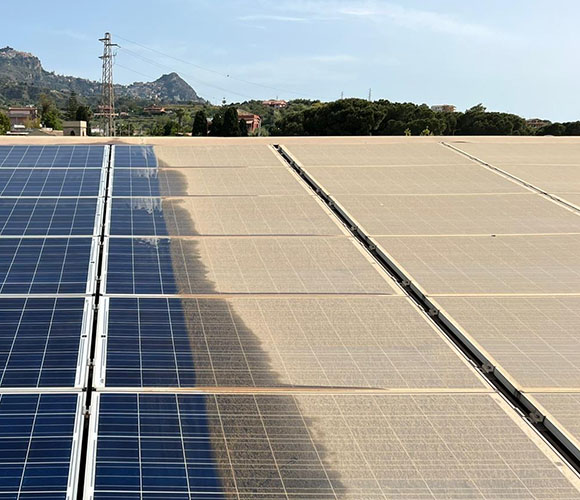
\includegraphics[width=0.5\textwidth]{Images/pannelli_sporchi2.jpg}
	\end{figure}\\
	Per affrontare il problema della pulizia, il proprietario dell'impianto può scegliere se rivolgersi ad imprese specializzate che effettuano pulizia a domicilio oppure prevenire il problema scegliendo di installare pannelli autopulenti di ultima generazione. Entrambe queste soluzioni hanno però dei limiti: per quanto riguarda la prima possibilità è l'utente stesso che deve accorgersi di quando sopraggiunge il momento opportuno per eseguire la pulizia e deve mobilitarsi per contattare l'impresa adeguata per un costo che in media varia tra i 100\euro e 300\euro.\\
	Parlando invece di pannelli autopulenti, essi sono un arma a doppio taglio. Possono essere realizzati sfruttando diverse tecnologie che spaziano dall'impiego di materiali con attrito estremamente ridotto, sfruttando l'acqua piovana per lavare via la sporcizia, all'uso di impulsi elettrici per far letteralmente "saltare via" le impurità dalla superficie. Tuttavia, mentre queste tecnologie di ultimissima generazione sono fuori dalla portata dei molti, l'uso di materiali dall'attrito ridotto (oltre che essere caratterizzati da costi di acquisto superiori rispetto  a pannelli tradizionali) comporta una forte dipendenza dalle precipitazioni atmosferiche che, per di più, possono anche risultare controproducenti dal momento che in aree cittadine, o in generale più inquinate, l'acqua piovana andrebbe a depositare ulteriori rifiuti sulla superficie.\\
	\section{Soluzione proposta}
	La nostra proposta consiste nel fornire un sistema completamente automatizzato per la pulizia dell'impianto fotovoltaico. L'idea di base è quella di monitorare costantemente l'efficienza energetica di ogni pannello in modo tale da rendersi conto quando non è più in grado di fornire adeguate prestazioni a causa dello sporco che vi si è depositato sopra. Quando l'efficienza scende sotto una certa soglia prestabilita dal proprietario; il nostro sistema è in grado di effettuare la pulizia usando l'adeguato detergente, reso disponibile in una piccola cisterna installata nello stabile, rilasciandola sul pannello.\\
	% immagine dell'impianto
	Questa soluzione consentirebbe al proprietario dell'impianto non solo si risparmiare notevolmente sul costo della pulizia, ma questa verrebbe effettuata automaticamente dal sistema senza che l'utente debba preoccuparsi di nulla.\\
	Il liquido adeguato per la pulizia della superficie è l'acqua osmotica, o osmotizzata, che può assere acquistata dall'utente al costo di circa 1 \euro/L in modo che egli possa occuparsi di mantenere attivo il sistema in completa autonomia, senza dover contattare un tecnico o un'impresa specializzata.\\\\
	La misurazione dell'efficienza energetica è realizzabile in modo relativamente semplice, infatti il nostro dispositivo dialoga direttamente con gli ottimizzatori: delle componenti già presenti all'interno dell'impianto fotovoltaico che, a intervalli di tempo regolari, raccolgono i report provenienti dai vari pannelli. Ciascun report contiene, tra le altre informazioni, anche l'efficienza energetica che può essere intercettata dal nostro dispositivo il quale ne tiene traccia. Questo metodo di misurazione è efficace poiché, piuttosto che sfruttare l'energia prodotta (che può variare a seconda delle condizioni atmosferiche), basandosi sull'efficienza questa esprime il rapporto tra l'energia generata e l'energia solare ricevuta; qualora il valore dovesse diminuire, significa che le prestazioni del pannello stanno diminuendo.
	% dire che la nostra idea è più economica delle alternative lo diciamo qui oppure nell'analisi del settore?
	\section{Il settore}
	\section{Il mercato e il cliente}
	\section{Modello di business}
	\section{Funzionamento del prodotto}
	\section{WBS e Prospetto di Gantt}
\end{document} 